\documentclass[10pt,aspectratio=169]{beamer}

% All the boilerplate is in raslides.sty
% Note that this also pulls in a custom vogtwidebar.sty
\usepackage{raslides}

\author{Ji\v{r}\'i Lebl}

\institute[OSU]{%
Departemento pri Matematiko de Oklahoma {\^S}tata Universitato}

\title{BA: 5.3}

\date{}

\begin{document}

\begin{frame}
\titlepage
\end{frame}

\begin{frame}
\begin{theorem}[1\textsu{st} form of the Fundamental Theorem of Calculus]
Let $F \colon [a,b] \to \R$ be continuous, differentiable
on $(a,b)$.
\pause
Let $f \in \sR[a,b]$ be such that $f(x) = F'(x)$ for $x \in
(a,b)$.
\pause
Then
\vspace*{-12pt}
\begin{equation*}
\int_a^b f = F(b)-F(a) .
\end{equation*}
\end{theorem}

\pause
\textbf{Proof:}
Let $P = \{ x_0, x_1, \ldots, x_n \}$ be a partition of $[a,b]$.

\pause
By MVT, $\forall$ $i$ find
$c_i \in (x_{i-1},x_i)$ s.t.
~$f(c_i) \Delta x_i = F'(c_i) (x_i - x_{i-1}) = F(x_i) - F(x_{i-1})$.

\pause
\medskip

\begin{center}
\scalebox{0.7}{
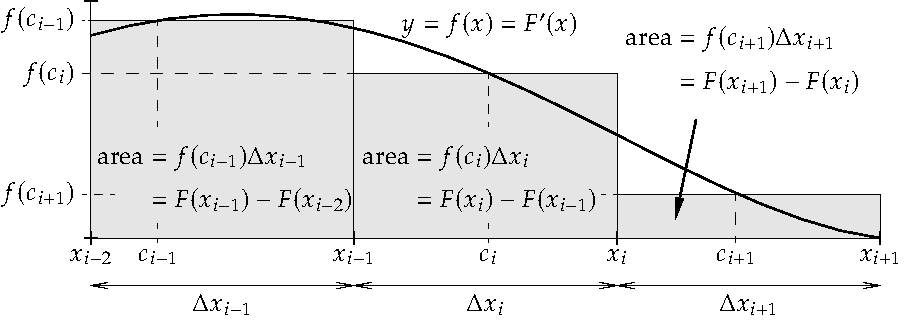
\includegraphics{../figures/fundthmfig}
}
\end{center}

\pause
The area of all
three shaded rectangles is $F(x_{i+1})-F(x_{i-2})$.

\end{frame}

\begin{frame}
Using the notation from the definition of the integral, \quad
$m_i \leq f(c_i) \leq M_i$ \quad $\forall i$.

\pause
\medskip

\thus \quad
$m_i \Delta x_i
\pause
\leq F(x_i) - F(x_{i-1})
\pause
\leq M_i \Delta x_i$
\quad
$\forall i$

\pause
\medskip

\thus \quad
$\displaystyle
\sum_{i=1}^n m_i \Delta x_i
\pause
\leq \sum_{i=1}^n \bigl(F(x_i) - F(x_{i-1}) \bigr)
\pause
\leq \sum_{i=1}^n M_i \Delta x_i$.

\pause
\medskip

\thus \quad
$\displaystyle
L(P,f) \leq F(b)-F(a) \leq U(P,f)$.

\pause
\medskip

\thus \quad
$\displaystyle
\underline{\int_a^b} f
\leq
F(b)-F(a)
\leq
\overline{\int_a^b} f$.

\pause
\medskip

$f$ is Riemann integrable
\pause
\wthus 
$\displaystyle \int_a^b f
\pause
=
\underline{\int_a^b} f
\pause
\leq
F(b)-F(a)
\pause
\leq
\overline{\int_a^b} f
\pause
=
\int_a^b f$.

\pause
\medskip

\thus  \quad
$\displaystyle \int_a^b f = F(b)-F(a)$.
\qed

\end{frame}

\begin{frame}

\textbf{Example:}
To compute
\begin{equation*}
\int_0^1 x^2 \,dx ,
\end{equation*}
\pause
notice $x^2$ is the derivative of $\frac{x^3}{3}$.

\pause
The fundamental theorem says
\begin{equation*}
\int_0^1 x^2 \,dx
\pause
=
\frac{1^3}{3}
-
\frac{0^3}{3}
= \frac{1}{3}.
\end{equation*}

\end{frame}

\begin{frame}

\begin{theorem}[2\textsu{nd} form of the Fundamental Theorem of Calculus]
Let $f \colon [a,b] \to \R$ be a Riemann integrable function.
\pause
Define
\begin{equation*}
F(x) \coloneqq \int_a^x f .
\end{equation*}
\pause
First, $F$ is continuous on $[a,b]$.
\pause
Second,
if $f$ is continuous at $c \in [a,b]$, then $F$ is differentiable at $c$
and $F'(c) = f(c)$.
\end{theorem}

\pause
\textbf{Proof:}
$f$ is bounded \wthus $\exists$ $M > 0$ s.t.  $\abs{f(x)} \leq M$ for all $x \in [a,b]$.

\pause
\medskip

If
$x,y \in [a,b]$ with $x > y$,
~~
$\displaystyle
\abs{F(x)-F(y)}
\pause
=
\abs{\int_a^x f - \int_a^y f}
\pause
=
\abs{\int_y^x f}
\pause
\leq
M\abs{x-y}$.

\pause
\medskip

Same holds if $x < y$.

\pause
\medskip

So $F$ is Lipschitz, thus continuous.

\end{frame}

\begin{frame}
Now suppose $f$ is continuous at $c$.

\pause
Fix $\epsilon > 0$.
\pause
Find $\delta > 0$ s.t.
for $x \in [a,b]$, $\abs{x-c} < \delta$, we have $\abs{f(x)-f(c)} < \epsilon$.

\pause
For such $x$, \quad
$f(c)-\epsilon < f(x) < f(c) + \epsilon$.

\pause
\medskip

\thus \quad
if $x > c$, then
~~
$\displaystyle
\bigl(f(c)-\epsilon\bigr) (x-c)
\pause
\leq
\int_c^x f
\pause
\leq
\bigl(f(c) + \epsilon\bigr)(x-c)$.

\pause
\medskip

If $c > x$, the inequalities reverse.

\pause
\medskip

\thus \quad if $x \not= c$, \quad
$\displaystyle
f(c)-\epsilon
\pause
\leq
\frac{\int_c^{x} f}{x-c}
\pause
\leq
f(c)+\epsilon$.

\pause
\medskip

$\displaystyle
\frac{F(x)-F(c)}{x-c}
\pause
=
\frac{\int_a^{x} f - \int_a^{c} f}{x-c}
\pause
=
\frac{\int_c^{x} f}{x-c}$

\pause
\medskip

\thus
\quad
$\displaystyle
\abs{\frac{F(x)-F(c)}{x-c} - f(c)} \leq \epsilon$.

\pause
\medskip
The result follows.
\qed
\end{frame}

\begin{frame}

\textbf{Remark:}
If $f$ is continuous on $[a,b]$,
\pause
then it is Riemann integrable,
\pause
$F$ is differentiable on all of $[a,b]$,
\pause
and $F'(x) = f(x)$ for
all $x \in [a,b]$.

\pause
\medskip

\textbf{Remark:}
2\textsu{nd} form of FTC still holds if for
$d \in [a,b]$, we define
\begin{equation*}
F(x) \coloneqq \int_d^x f .
\end{equation*}
\pause
Any point can be the base point.
\pause
\textbf{Proof:} Exercise.

\pause
\medskip

\textbf{Example:}
Define $f(x) \coloneqq -1$ if $x
< 0$, and $f(x) \coloneqq 1$ if $x \geq 0$.

\pause
Let $F(x) \coloneqq \int_0^x f$.
\pause
\qquad Not hard to see that $F(x) = \abs{x}$.

\pause
$f$ is discontinuous at $0$ and $F$ is not differentiable at $0$.

\pause
\medskip

The converse in the theorem does not hold.

\pause
Let $g(x) \coloneqq 0$ if $x \not= 0$, and $g(0) \coloneqq 1$.

\pause
Let $G(x) \coloneqq \int_0^x g$. \qquad
\pause
Then $G(x) = 0$ for all $x$.

\pause
$g$ is discontinuous at $0$, but $G'(0)$ exists and equals 0.

\end{frame}

\begin{frame}

\textbf{Remark on calculus:}
What is ``closed form''?

\pause
\medskip

Natural logarithm is just defined as
\begin{equation*}
\ln x \coloneqq \int_1^x \frac{1}{s}\,ds .
\end{equation*}

\pause
So is writing $\int_a^b \frac{1}{x} \,dx = \ln b-\ln a$ writing things in
closed form?

\pause
\medskip

Another common function defined by an integral
\begin{equation*}
\operatorname{erf}(x) \coloneqq \frac{2}{\sqrt{\pi}} \int_0^x e^{-s^2} \,ds .
\end{equation*}

\pause
\medskip

etc.

\end{frame}

\begin{frame}

\begin{theorem}[Change of variables or $u$-substitution]
Let $g \colon [a,b] \to \R$ be continuously differentiable,
\pause
$f \colon [c,d] \to \R$ continuous,
\pause
and suppose
$g\bigl([a,b]\bigr) \subset [c,d]$.
\pause
Then
\vspace*{-6pt}
\begin{equation*}
\int_a^b f\bigl(g(x)\bigr)\, g'(x)\, dx =
\int_{g(a)}^{g(b)} f(s)\, ds .
\end{equation*}
\end{theorem}

\pause
\textbf{Proof:}
$g$, $g'$, and $f$ are continuous
\pause
\wthus $f\bigl(g(x)\bigr)\,g'(x)$
is continuous on $[a,b]$,

\pause
thus Riemann integrable.
\pause
\quad
Also, $f$ integrable on every subinterval of $[c,d]$.

\pause
\medskip

Define $F \colon [c,d] \to \R$ by~
$F(y) \coloneqq \int_{g(a)}^{y} f(s)\,ds$.

\pause
By 2\textsu{nd} form of FTC, $F$ is differentiable and $F'(y) = f(y)$.

\pause
Chain
rule \wthus
$\bigl( F \circ g \bigr)' (x)
\pause
=
F'\bigl(g(x)\bigr) g'(x)
\pause
=
f\bigl(g(x)\bigr) g'(x)$.

\pause
$F\bigl(g(a)\bigr) = 0$ and
the 1\textsu{st} form of FTC implies

\pause
\medskip

$\displaystyle
\int_{g(a)}^{g(b)} f(s)\,ds
\pause
= F\bigl(g(b)\bigr)
\pause
= F\bigl(g(b)\bigr)-F\bigl(g(a)\bigr)
$

\pause
\qquad
$\displaystyle
=
\int_a^b 
\bigl( F \circ g \bigr)' (x) \,dx
\pause
=
\int_a^b 
f\bigl(g(x)\bigr) g'(x)
\,dx$.
\qed
\end{frame}

\begin{frame}

\textbf{Example:}
The derivative of $\sin(x)$ is $\cos(x)$.
\pause
Using $g(x) \coloneqq x^2$,
\pause
\begin{equation*}
\int_0^{\sqrt{\pi}} x \cos(x^2) \, dx
\pause
= \int_0^\pi \frac{\cos(s)}{2} \, ds
\pause
=
\frac{1}{2}
\int_0^\pi \cos(s) \, ds
\pause
=
\frac{
\sin(\pi) - \sin(0)
}{2}
\pause
=
0 .
\end{equation*}

\pause
\medskip

\textbf{Example:}
Consider
\quad
$\displaystyle
\int_{-1}^{1} \frac{\ln \abs{x}}{x} \,dx$.

\pause
\medskip

Tempting to take $g(x) \coloneqq \ln \abs{x}$.
\pause
Compute $g'(x) =
\nicefrac{1}{x}$ and try to write
\begin{equation*}
\int_{-1}^{1} \frac{\ln \abs{x}}{x} \,dx
\pause
=
\int_{g(-1)}^{g(1)} s \,ds
\pause
= 
\int_{0}^{0} s \,ds = 0. 
\end{equation*}
\pause
\vspace*{-42pt}
\begin{center}
{\color{red}
\Huge XXXXXXXXXX
}
\end{center}
This is \textbf{incorrect!}

\pause
\medskip

1) $\frac{\ln \abs{x}}{x}$ is not continuous on $[-1,1]$.

\pause
\medskip

2) $\frac{\ln \abs{x}}{x}$ is not even Riemann integrable on $[-1,1]$
(it is unbounded).

\pause
\medskip

$\int_{-1}^{1} \frac{\ln \abs{x}}{x} \,dx$
simply does not make sense!

\pause
\medskip

3) $g$ is not continuous on $[-1,1]$, let alone continuously differentiable.

\end{frame}

\begin{frame}

\textbf{Exercise:}
Suppose $F \colon [a,b] \to \R$ is continuous and differentiable
on $[a,b] \setminus S$, where $S$ is a finite set.
\pause
Suppose there
exists an $f \in \sR[a,b]$ such that $f(x) = F'(x)$ for $x \in [a,b]
\setminus S$.
\pause
Show that
$\int_a^b f = F(b)-F(a)$.

%\pause
%\medskip
%
%\textbf{Exercise:}
%Let $f \colon [a,b] \to \R$ be continuous.  Let $c \in [a,b]$
%be arbitrary.
%\pause
%Define
%\begin{equation*}
%F(x) \coloneqq \int_c^x f .
%\end{equation*}
%\pause
%Prove that $F$ is differentiable and that $F'(x) = f(x)$ for all $x \in
%[a,b]$.

\pause
\medskip

\textbf{Exercise:}
Let $f \colon [a,b] \to \R$ be continuous and $\epsilon > 0$.
For $x \in [a+\epsilon,b-\epsilon]$, define
\begin{equation*}
g(x) \coloneqq \frac{1}{2\epsilon} \int_{x-\epsilon}^{x+\epsilon} f .
\end{equation*}
\begin{enumerate}[a)]
\item\pause
Show that $g$ is differentiable and find the derivative.
\item\pause
Let $f$ be differentiable and fix $x \in (a,b)$ (let $\epsilon$
be small enough).  What happens to $g'(x)$ as $\epsilon$ gets smaller?
\item\pause
Find $g$ for $f(x) \coloneqq \abs{x}$, $\epsilon = 1$ (you can assume 
$[a,b]$ is large enough).
\end{enumerate}

\end{frame}

\end{document}
